
\documentclass[border=8pt, multi, tikz]{standalone} 
\usepackage{import}
\subimport{../layers/}{init}
\usetikzlibrary{positioning}
\usetikzlibrary{3d} %for including external image 

\def\ConvColor{rgb:yellow,5;red,2.5;white,5}
\def\ConvReluColor{rgb:yellow,5;red,5;white,5}
\def\PoolColor{rgb:red,1;black,0.3}
\def\PoolReluColor{rgb:red,2;black,0.3}
\def\UnpoolColor{rgb:blue,2;green,1;black,0.3}
\def\FcColor{rgb:blue,5;red,2.5;white,5}
\def\BatchNcolor{rgb:blue,19;green,69;red,139}
\def\FcReluColor{rgb:blue,5;red,5;white,4}
\def\SoftmaxColor{rgb:magenta,2.5;black,7}   
%\def\SoftmaxReluColor{rgb:magenta,5;black,7}   

\newcommand{\copymidarrow}{\tikz \draw[-Stealth,line width=0.8mm,draw={rgb:blue,4;red,1;green,1;black,3}] (-0.3,0) -- ++(0.3,0);}

\begin{document}
\begin{tikzpicture}
    \tikzstyle{connection}=[ultra thick,every node/.style={sloped,allow upside down},draw=\edgecolor,opacity=0.7]
    \tikzstyle{copyconnection}=[ultra thick,every node/.style={sloped,allow upside down},draw={rgb:blue,4;red,1;green,1;black,3},opacity=0.7]

    \node[canvas is zy plane at x=0] (temp) at (-1,0,0) {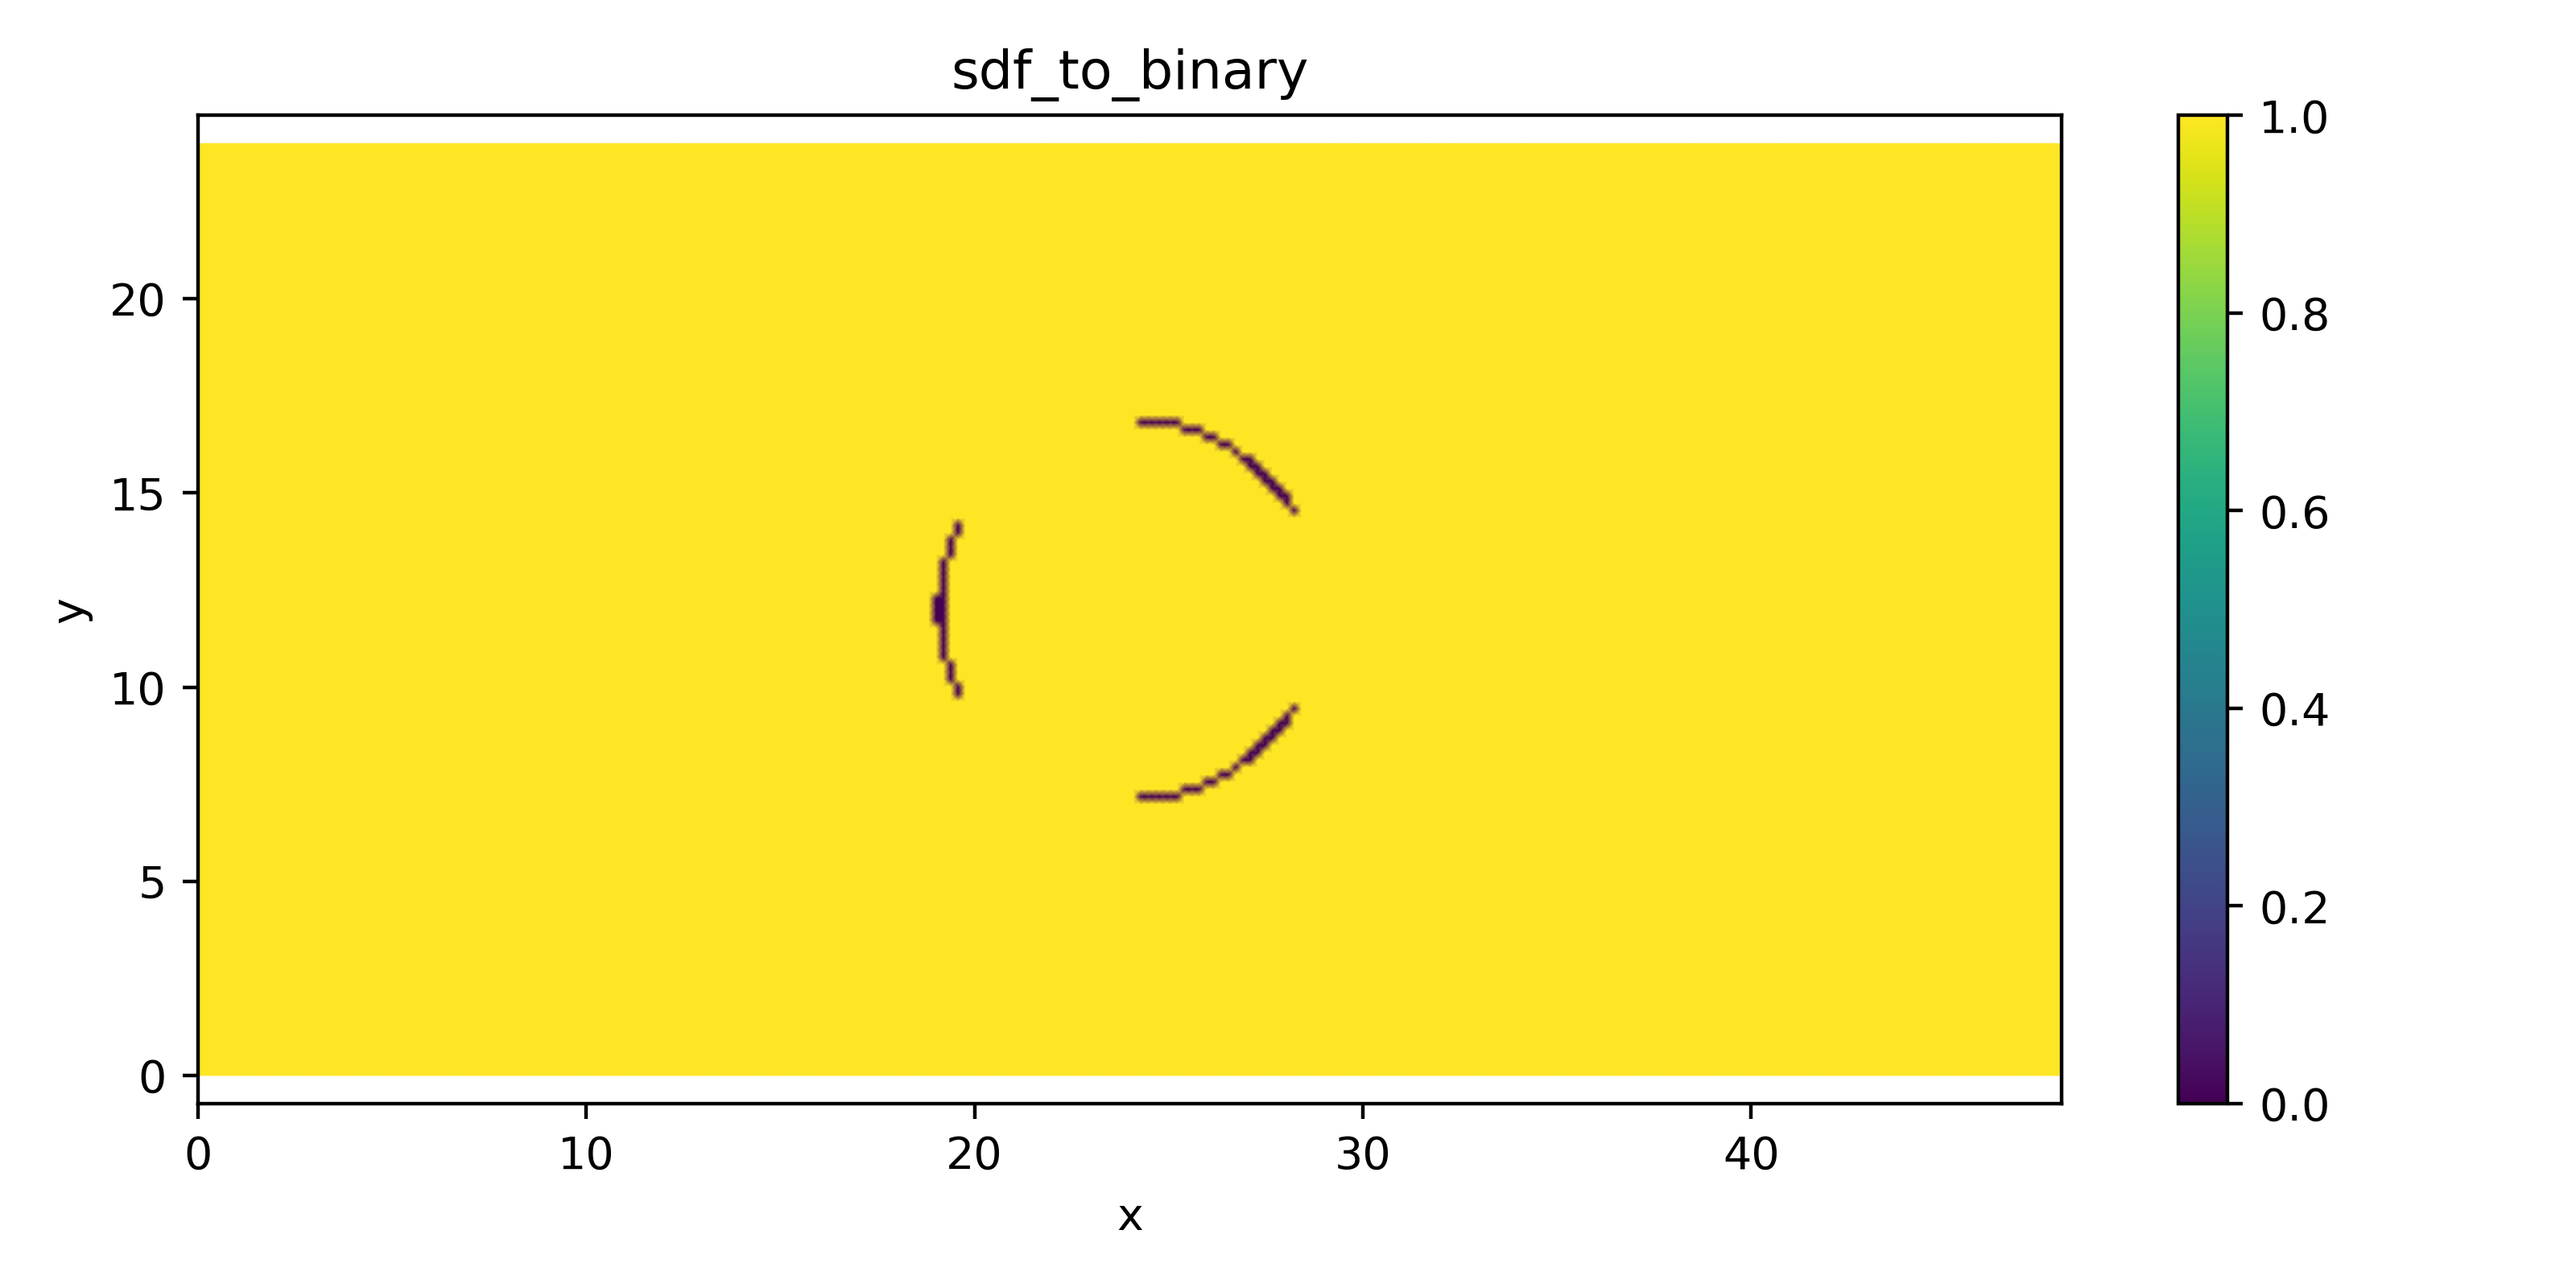
\includegraphics[width=16cm,height=8cm]{../inputs/sdf_to_binary.png}};

    \pic[shift={ (2,0,0) }] at (0,0,0)
    {RightBandedBox={
                name=conv1,
                caption=conv1,
                xlabel={{8, }},
                ylabel= 128,
                zlabel=256,
                fill=\ConvColor,
                bandfill=\ConvReluColor,
                height=32,
                width= 16,
                depth=64
            }
    };

    \pic[shift={ (0,0,0) }] at (conv1-east)
    {Box={
                name=batch1,
                caption= ,
                fill=\BatchNcolor,
                opacity=0.5,
                height=32,
                width=1,
                depth=64
            }
    };

    \pic[shift={ (0,0,0) }] at (batch1-east)
    {Box={
                name=pool1,
                caption=,
                xlabel={{, }},
                ylabel=,
                zlabel=,
                fill=\PoolColor,
                opacity=0.5,
                height=16,
                width=1,
                depth=32
            }
    };

    \pic[shift={ (2,0,0) }] at (pool1-east)
    {RightBandedBox={
                name=conv2,
                caption=conv2,
                xlabel={{16, }},
                ylabel= 64,
                zlabel=128,
                fill=\ConvColor,
                bandfill=\ConvReluColor,
                height=16,
                width= 8,
                depth=32
            }
    };

    \pic[shift={ (0,0,0) }] at (conv2-east)
    {Box={
                name=batch2,
                caption= ,
                fill=\BatchNcolor,
                opacity=0.5,
                height=16,
                width=1,
                depth=32
            }
    };

    \draw [connection]  (pool1-east)    -- node {\midarrow} (conv2-west);

    \pic[shift={ (0,0,0) }] at (batch2-east)
    {Box={
                name=pool2,
                caption=,
                xlabel={{, }},
                ylabel=,
                zlabel=,
                fill=\PoolColor,
                opacity=0.5,
                height=8,
                width=1,
                depth=16
            }
    };

    \pic[shift={ (2,0,0) }] at (pool2-east)
    {RightBandedBox={
                name=conv3,
                caption=conv3,
                xlabel={{32, }},
                ylabel= 32,
                zlabel=64,
                fill=\ConvColor,
                bandfill=\ConvReluColor,
                height=8,
                width= 5,
                depth=16
            }
    };

    \pic[shift={ (0,0,0) }] at (conv3-east)
    {Box={
                name=batch3,
                caption= ,
                fill=\BatchNcolor,
                opacity=0.5,
                height=8,
                width=1,
                depth=16
            }
    };

    \draw [connection]  (pool2-east)    -- node {\midarrow} (conv3-west);

    \pic[shift={ (0,0,0) }] at (batch3-east)
    {Box={
                name=pool3,
                caption=,
                xlabel={{, }},
                ylabel=,
                zlabel=,
                fill=\PoolColor,
                opacity=0.5,
                height=4,
                width=1,
                depth=8
            }
    };

    \pic[shift={ (2,0,0) }] at (pool3-east)
    {RightBandedBox={
                name=conv4,
                caption=conv4,
                xlabel={{64, }},
                ylabel= 16,
                zlabel=32,
                fill=\ConvColor,
                bandfill=\ConvReluColor,
                height=4,
                width= 4,
                depth=8
            }
    };

    \pic[shift={ (0,0,0) }] at (conv4-east)
    {Box={
                name=batch4,
                caption= ,
                fill=\BatchNcolor,
                opacity=0.5,
                height=4,
                width=1,
                depth=8
            }
    };

    \draw [connection]  (pool3-east)    -- node {\midarrow} (conv4-west);

    \pic[shift={ (0,0,0) }] at (batch4-east)
    {Box={
                name=pool4,
                caption=,
                xlabel={{, }},
                ylabel=,
                zlabel=,
                fill=\PoolColor,
                opacity=0.5,
                height=2,
                width=1,
                depth=4
            }
    };

    \pic[shift={ (2,0,0) }] at (pool4-east)
    {RightBandedBox={
                name=conv5,
                caption=conv5,
                xlabel={{128, }},
                ylabel= 8,
                zlabel=16,
                fill=\ConvColor,
                bandfill=\ConvReluColor,
                height=2,
                width= 6,
                depth=4
            }
    };

    \pic[shift={ (0,0,0) }] at (conv5-east)
    {Box={
                name=batch5,
                caption= ,
                fill=\BatchNcolor,
                opacity=0.5,
                height=2,
                width=1,
                depth=4
            }
    };

    \draw [connection]  (pool4-east)    -- node {\midarrow} (conv5-west);

    \pic[shift={ (0,0,0) }] at (batch5-east)
    {Box={
                name=pool5,
                caption=,
                xlabel={{, }},
                ylabel=,
                zlabel=,
                fill=\PoolColor,
                opacity=0.5,
                height=1,
                width=1,
                depth=2
            }
    };

    \pic[shift={ (2,0,0) }] at (pool5-east)
    {RightBandedBox={
                name=conv6,
                caption=conv6,
                xlabel={{256, }},
                ylabel= 4,
                zlabel=8,
                fill=\ConvColor,
                bandfill=\ConvReluColor,
                height=1,
                width= 10,
                depth=2
            }
    };

    \pic[shift={ (0,0,0) }] at (conv6-east)
    {Box={
                name=batch6,
                caption= ,
                fill=\BatchNcolor,
                opacity=0.5,
                height=1,
                width=1,
                depth=2
            }
    };

    \draw [connection]  (pool5-east)    -- node {\midarrow} (conv6-west);

    \pic[shift={ (0,0,0) }] at (batch6-east)
    {Box={
                name=pool6,
                caption=,
                xlabel={{, }},
                ylabel=,
                zlabel=,
                fill=\PoolColor,
                opacity=0.5,
                height=0,
                width=1,
                depth=1
            }
    };

    \pic[shift={(2.5,0,0)}] at (pool6-east)
    {Box={
                name=flatten_1,
                caption=flatten,
                xlabel={{" ","dummy"}},
                zlabel=2048,
                fill=\SoftmaxColor,
                opacity=0.8,
                height=1,
                width=1,
                depth=64
            }
    };

    \draw [connection]  (pool6-east)    -- node {\midarrow} (flatten_1-west);

    \pic[shift={(1.5,0,0)}] at (flatten_1-east)
    {Box={
                name=hidden1,
                caption=hidden1,
                xlabel={{" ","dummy"}},
                zlabel=512,
                fill=\SoftmaxColor,
                opacity=0.8,
                height=1,
                width=1,
                depth=16
            }
    };

    \draw [connection]  (flatten_1-east)    -- node {\midarrow} (hidden1-west);

    \pic[shift={(1.5,0,0)}] at (hidden1-east)
    {Box={
                name=hidden2,
                caption=hidden2,
                xlabel={{" ","dummy"}},
                zlabel=128,
                fill=\SoftmaxColor,
                opacity=0.8,
                height=1,
                width=1,
                depth=4
            }
    };

    \draw [connection]  (hidden1-east)    -- node {\midarrow} (hidden2-west);

    \pic[shift={(1.5,0,0)}] at (hidden2-east)
    {Box={
                name=output,
                caption=Output,
                xlabel={{" ","dummy"}},
                zlabel=1,
                fill=\SoftmaxColor,
                opacity=0.8,
                height=1,
                width=1,
                depth=1
            }
    };

    \draw [connection]  (hidden2-east)    -- node {\midarrow} (output-west);

\end{tikzpicture}
\end{document}
